\documentclass[12pt]{article}
\usepackage{amsmath}
\usepackage{amssymb}
\usepackage{amsthm}
\usepackage{color}
\usepackage{graphicx}
\usepackage[round]{natbib}
\usepackage{xspace}
\usepackage{hyperref}
\usepackage{hypernat}
\linespread{1.7}


\newcommand{\avec}{\ensuremath{\vec{a}}\xspace}
\newcommand{\avecopt}{\ensuremath{\vec{a}^\prime}\xspace}
\newcommand{\aopt}{\ensuremath{a^\prime}\xspace}
\newcommand{\Qmat}{\ensuremath{\mathbf{Q}}\xspace}

\includeonly{abstract,introduction,methods}

\title{A phylogenetic and population genetic model of amino acid substitution}
\author{}
\begin{document}
\maketitle
%%%%%%%%%%%%%%%%%%%%%%%%%%%%%%%%%%%%%%%%%%%%%%%%%%%%%%%%
\section{Abstract}
We introduce a new, mechanistic Markov model for studying the evolution of amino acid sequences within a phylogenetic context.
Our model links together genotype, phenotype, and fitness of proteins, by calculating the fixation probability of a newly arisen mutant using a model of allele substitution from population genetics. 
As a result, our model explicitly includes the effects of mutation bias, genetic drift, and natural selection favoring an optimal amino acid sequence for a given protein.
We assume that the strength of purifying selection is a function of the physiochemical differences between a given amino acid and the optimal amino acid for the site, how a protein's functionality declines with this distance, and the target expression level of the gene.
Analysis of a multi-locus yeast data set using AIC shows that our new model provides a substantially better fit to data than the standard empirical models and allows researchers to estimate biologically meaningful parameters such as the sensitivity of a protein's function to an amino acid substitution and the optimal amino acids at a given site.
Further, because our model is based on explicit models of various biological processes, unlike empirical models it can easily be modified in the future to include other important biological phenomena such as selection on codon usage or test alternative hypotheses about the relationship between amino acid sequence and protein functionality.

\newpage
\tableofcontents
\section{Introduction}

TO ADD: Importance of building accurate model for protein evolution. \\

In phylogenetics, models for evolution of protein-encoding sequences are usually formulated at three levels: mono-nucleotide level in DNA \citep[e.g., see][]{jukes1969evolution, kimura1980, felsenstein1981evolutionary, hasegawa1985dating}, codon level \citep[see][]{GoldmanYang1994,muse1994,yang1998models,yang2008mutation}, and amino acid (AA) level \citep[see][]{kishino1990maximum}.
The nucleotides, codons, or amino acids are assumed to evolve independently.
DNA- and codon-based models use more data and are often the most powerful in terms of their ability to distinguish between closely related sequences. 
Of these two, codon-based models use all the information in DNA and know the product of amino acid in addition. On the other hand, AA-based models ignore synonymous differences between sequences by focusing not on the codons themselves but the amino acids they code for. 
Since synonymous codon usage is largely driven by mutation bias in low expression genes and selection on translational efficiency for high expression genes \citep[see][]{Gilchrist2007}[{\color{blue} CHECK CITATIONS, add CUB citation}], ignoring this aspect of the data has the advantage of reducing the noise in sequence data for low expression genes but at the cost of losing potentially useful information held in the high expression genes.

Based on how the substitution rates are formulated, models of amino acid substitution fall into two categories: empirical models and mechanistic models. 
In empirical models, the substitution rates are based solely on analysis of large quantities of sequence data complied from databases.
Commonly used models in this category include  Dayhoff \citep{dayhoff1978model}, JTT \citep{jones1992rapid}, WAG \citep{whelan2001general}, LG \citep{lg2008improved} for nuclear proteins; mtREV, MTMAM \citep{adachi1996model, yang1998models} for mitochondrial proteins; and cpREV \citep{adachi2000plastid} model for chloroplast proteins, etc. \citep[see][]{cao1994phylogenetic, henikoff1992amino, gonnet1992exhaustive} 
In contrast, mechanistic models are formulated based on the hypothesized biological processes thought to drive sequence evolution, such as mutation bias in DNA, translation of codons into amino acids, and natural selection.

%Mike
The Goldman and Yang (1994) model, GY, is a  codon level mechanistic model, which includes mutation and purifying selection for the aa of the ( ) of a lineage, transition vs. transversion bias. The strength of purifying selection is incorporated by multiplying the substitution rate by a factor $\exp (- d_{aa_i,aa_j}/V)$ where $d_{aa_i, aa_j}$ is the physiochemical distance between amino acids $aa_i$ and $aa_j$ defined by \citet{grantham1974} (i.e.~Grantham Distances) and $V$ is a parameter representing the variability of the gene or its tendency to undergo non-synonymous substitution. ({\color{blue} V scales sensitivity to $d$, as $V \rightarrow 0$ infinite selection, and as $V \rightarrow \infty$ there is no selection.})
The model in common use is a simplified version of this model that ignores the effect of selection.
\citet{yang1998models} implemented a few mechanistic models {\color{blue} vague, are there variations of GY?} on the codon level and found from analysis of mitochondrial genomes of 20 mammalian species that they fit the data better than empirical models ({\color{blue} based on -loglikelihood or AIC or something else?}). 
One trait common to most phylogenetic models, whether empirical or mechanistic, and including the GY model, is time reversibility. 
In time-reversible models, the relative substation rate $q_{ij}$ from state $i$ to state $j$ is assumed to satisfy the detailed balance condition $\pi_{i} q_{ij} = \pi_j q_{ji}$ for any $i \ne j$.
While time reversibility provides substantial mathematical and computational advantages, it is difficult to interpret biologically. This, surprisingly, has been largely ignored by the phylogentics community. ({\color{blue} CITATIONS of exceptions?})


%\citet{GoldmanYang1994} implemented a mechanistic model (GY) at the level of codons and explicitly modeled the biological processes involved, including different mutation rates between nucleotides (transition vs. transversion bias), the translation of the codon triplet into an amino acid (synonymous vs. non-synonymous rates), and the acceptance or rejection of the amino acid due to selective pressure on the protein. 
%The selective restraints at the amino acid level was accounted for by multiplying the substitution rate by a factor $\exp (d_{aa_i,aa_j}/V)$ where $d_{aa_i, aa_j}$ is the distance between amino acids $aa_i$ and $aa_j$ given by \citet{grantham1974} (i.e.~Grantham Distances) and $V$ is a parameter representing the variability of the gene or its tendency to undergo non-synonymous substitution.
%The model in common use is a simplified version of this model that ignores the effect of selection.
%\citet{yang1998models} implemented a few mechanistic models on the codon level and found from analysis of mitochondrial genomes of 20 mammalian species that they fit the data better than empirical models.

For example, if amino acid $i$ is favored by natural selection, then in the absence of mutation bias we expect the substitution rate from state $j$ to $i$ to be faster then the reverse. 
While mutation bias can alter this requirement when selection is weak, it can only do so when the assumption of time reversibility is violated. ({\color{blue} JJ - is this true? substitution rates are different from exchange rates, even in time-reversible models. Under time-reversible model, the higher equilibrium state frequency indicates higher mutation rate to this state. In the discussion follows, consider the case where amino acid $i$ has a higher equilibrium frequency than amino acid $j$, even if in the exchange rate matrix synonymous rates are bigger than non synonymous rates, it's still possible that the substation rates reflect the ``optimality'' of amino acids. } )
For example, consider a time-reversible codon substitution model where synonymous substitutions occur at a faster rate than non-synonymous substitutions.
For any given state of the system, such a model implies that the current amino acid is optimal since synonymous substitutions occur at a faster rate than non-synonymous ones.
However, once a non-synonymous substitution has occurred (and as time goes to infinity it will),  the time reversible aspects of the model now imply that the new state is the optimal state and the old state is sub-optimal.
Thus, the only reasonable way to interpret such a time-reversible model is that the substitution matrix is actually describing the rate at which the optimal state switches at a given site and that once such a switch has occurred the system instantaneously shifts to the new state.
If, in contrast, one were to assume the converse, that non-synonymous substitution occur at a faster rate than synonymous, then the interpretation of time-reversible models becomes even more problematic from a biological perspective.
In such a scenario, not only is the optimal state constantly changing, the current state of any given site is always sub-optimal.

While time-reversible models have played an important role in molecular phylogenetics for the last several decades \citep{tavare1986} {\color{blue} wrong citation},  in order to model natural selection and mutation bias in a realistic manner the assumption of time reversibility must be relaxed.
In this study we develop an amino-acid based model in which we assume that for each individual site $i$ of a protein there is a corresponding optimal amino acid $a'_i$.
The optimal state can be assigned or, as we demonstrate, estimated from the data itself.
As with the GY model, we assume that the substitution rate between amino acids at a given site is a function of their Grantham distances from optimal amino acids and, assume genes can vary in their sensitivities to such deviation from optimal amino acids.
Here the sensitivity to amino acid changes is calculated using a cost-benefit framework we have developed previously for studying the evolution codon usage bias \citep{Gilchrist2007, gilchrist2009genetics,ShahGilchrist2011pnas}.
Furthermore, unlike most models in phylogenetics, we define the relative fitness of a phenotype, which is a given amino acid sequence, explicitly.
We then use a model from population genetics to calculate the substitution rate between any two genotypes by explicitly taking into account the fitness differences between them as well as the effects of mutation bias and genetic drift.
We use AIC to evaluate our model and alternative models by fitting them to the \citet{rokas2003nature}'s data set of 106 genes sequenced from 8 different species of yeast.
When fitting our model, we estimate the phylogenies of the yeast species, the Grantham sensitivity $g$ of a gene (roughly comparable to $1/V$ in the GY model), as well as the optimal amino acid $\avecopt$ for each site within a coding sequence.
We compare our model's fit to the Rokas data with other commonly used AA-based models using AIC criterion \citep{akaike1973information, akaike1974new, akaike1981likelihood}. [LIST MODELS] Our model is similar to GY model in that grantham distance is used, but we include the effect of natural selection explicitly, and allow for different substitution matrices depending on which amino acid is optimal.

Our results show that even with our most parameter rich model in which we estimate the optimal amino acid at every site, thereby introducing tens of thousands of additional parameters, our model still does a substantially better job fitting the Rokas dataset.
So although the computational cost of our model is greater than most time reversible models,  our ability to fit the phylogenetic data and extract biologically meaningful information is substantially greater than other models.
Furthermore, because our approach explicitly links genotype to phenotype, phenotype to fitness, and fitness to fixation rate, the biological assumptions underlying our model are clearly stated and incorporation of additional biological factors, such as selection on codon usage bias, is much more straighforward.
 


\section{Methods \& Materials}
In this study we use a series of continuous time Markov models with amino acid and gene specific parameterizations to describe the process of amino acid substitution for a given protein in a lineage. 

Our approach, is applicable to any homologous protein-coding DNA sequence dataset where any gaps have been removed.
In our model we assume that there is an optimal amino acid for any given site.
The strength of natural selection for the optimal amino acid is a function of the gene's expression level, the physiochemical properties of a given amino acid, and the sensitivity of the gene's functionality to changes in these properties.
It {\color{blue} what can vary?} can vary between genes and different sites in a gene. ({\color{blue} in current implementation sensitivity does not vary within a gene})
As a result, for each of 20 natural amino acids as optimal we have a $20 \times 20$ substation rate matrix with the same 20 amino acids as its states. 

Conceptually the substitution process consists of two steps. 
First, a given amino acid $i$ mutates to amino acid $j$, the rate of which depends on the mutation rates between nucleotides and the structure of the genetic code. 
Second, the newly arisen allele becomes fixed in the population with certain probability, which is based on the models from population genetics and includes the effects of natural selection and genetic drift. 
Therefore, when the optimal amino acid is $k$ the substitution rate matrix can be written as $Q_{i,j}^{(k)}=M_{i,j}F_{i,j}^{(k)}$ for $i \ne j$, where $M$ is the $20 \times 20$ mutation rate matrix between amino acids and $F$ is the $20 \times 20$ matrix of fixation probabilities. 
Note that $F$, but not $M$, depends on optimal amino acid $k$ for a given site. 
As usual the row sums of $Q$ equal $0$ and the matrix of substitution probabilities after time $t$ is $P^{(k)} = \exp (Q^{(k)}t)$

\subsection*{Calculating the Mutation Rate Matrix $M$}
We use a time reversible model for mutation between amino acids, i.e. $\pi_i M_{i,j} = \pi_j M_{j,i}$ where $\pi_i$ is the equilibrium frequency of the state $i$.
For all time reversible models, the substitution rate matrix can be written as $M=S\Pi$ where $S$ is a symmetric matrix called the exchange rate matrix and $\Pi$ is the diagonal matrix of base frequencies $\pi_i$'s of the states. The model is formulated at the amino acid level, so the calculation of $M$ involves 2 steps.


We begin with finding the mutation rate matrix between $61$ sense codons. 
For simplicity we assume that the mutations occur independently between nucleotides within a codon, and denote the mutation rate matrix for nucleotides by $M_{\nu}$. 
For codons that differ only by one nucleotide, the rate between codons is equal to the rate between the said pair of nucleotides.
For all other codons, since the changes involving two or more nucleotides during time $\Delta t$ have probabilities on the order of $\Delta t^2$, their mutation rates are set to $0$.
Therefore the $61 \times 61$ mutation rate matrix is rather sparse.


Second, from this codon level mutation rate matrix we can obtain $20 \times 20$ amino acid exchange rate matrix $S_{aa}$ by grouping together the synonymous codons for each amino acid. 
For simplicity, the synonymous codon frequencies for any given amino acid are assumed to be the same. 
Following the approach developed by Yang (MBE 1998), $S_{aa}$ for a reversible Markov process of amino acid mutation has entries:
\[(S_{aa})_{ij} = \frac{\sum_{u \in I} \sum_{v \in J} \pi_u \pi_v s_{uv}}{\pi_I \pi_J}\]
where $i$ and $j$ are two different amino acids, $I$ and $J$ are the corresponding sets of synonymous codons for $i$ and $j$ correspondingly, i.e. $c_u = i$ for $u\in I$ and $c_v = j$ for $v \in J$; $\pi_J = \sum_{v \in J} \pi_v$ is the equilibrium frequency of amino acid $j$ by combining the frequencies of synonymous odors for it; and $s_{uv}$ is the exchange rate between codons $u$ and $v$. 
The matrix $S_{aa}$ obtained in this way is symmetric, and we can find the mutation rate matrix by $(M)_{ij} = (S_{aa})_{ij} \pi_J$.\\

%------------------MIKE (start)-------------------------\\
%For simplicity, in this study we assume an underlying time reversible model of mutation. 
%In order to calculate the terms of this matrix, we first assume that mutations occur independently between nucleotides within a codon.
%For codons that differ by only one nucleotide, the mutation rate between codon $i$ and $j$ is equal to the mutation rate between these nucleotide.
%For all other codons, because changes involving two or more nucleotides during time $\Delta t$ will have probabilities on the order of $\Delta t^2$, we set their mutation rates to 0.
%
%For simplicity, we also assume that synonymous codon frequency for any given amino acid is uniform.
%Therefore, the equilibrium mutation rates between amino acids only depend on the frequencies of amino acids.
%This assumption of uniform codon usage could be altered by using a codon, rather than an amino acid, level model.
%
%
%For all time reversible models, the substitution rate matrix is a product of a symmetric matrix $S$ and the the base frequencies of different states: $Q = S\Pi$, where $S$ is called the exchange rate matrix and $\Pi$ is a diagonal matrix of the base frequencies.
%The mutation rate matrix for 20 amino acids are derived from the $4 \times 4 $ exchange rate matrix for nucleotides.
%This reduces the number of mutation rate parameters used to generate $S$ from 190 to 6.
%
%Thus, from $61 \times 61$ codon level mutation rate matrix we can obtain $20 \times 20$ amino acid exchange rate matrix $M$ by grouping together the synonymous codons for each amino acid.
%For example, suppose the sets of synonymous codons for amino acids $i$ and $j$ are $I$ and $J$ correspondingly, i.e. $c_u = i$ for $u \in I$, and $c_v = j$ for $v \in J$.
%Combining synonymous codons $J$ into one state, we have $\pi_J = \sum_{v \in J} \pi_v$ as the equilibrium frequency of amino acid $j$.
%The exchange rate matrix for a reversible Markov process of amino acid mutation $S$ has entries:
%\[\mu_{IJ} = \sum_{u \in I} \sum_{v \in J} \pi_u \pi_v s_{uv} / (\pi_I \pi_J)\]
%\noindent
%And $q_{IJ} = s_{IJ} \pi_J$ with $s_{IJ}  = s_{JI}$ constitutes the mutation rate matrix $M$.
%For detailed derivation see Yang(MBE 1998). [CAN'T YOU JUST SAY WE FOLLOW THE APPROACH DEVELOPED BY YANG 1998?  NO MATTER WHAT, WE SHOULD MENTION THIS PAPER EARLIER. -YES, I AGREE.]
%The mutation process is time reversible, i.e. $\pi_I \mu_{IJ} = \pi_J M_{JI}$ is satisfied for all $1 \leq I,J \leq 20$.
%[THIS SECTION STILL NEEDS WORK]\\
%------------------MIKE (end)-------------------------
\subsection*{Calculating the Fixation Probability Matrix $F$}
While the mutation rate matrix $M$ accounts for the effects of the structure of the genetic code and variation in mutation rates on the generation of new alleles,  $F$ describes the probabilities of any such mutation going to fixation.

Modeling the relationship between amino acid sequence and protein function is a complex and challenging problem [CITATION].
No general techniques that accurately and reliably predict a protein's structure, much less function, currently exist.
However, empirical data suggests that the effect of an amino acid on a protein's function depends largely on its physiochemical properties.
Therefore, we assume that for each site $i$ of the protein there is an optimal amino acid $k_i$.
If a protein consists solely of the optimal amino acids at all sites then it is defined to have 100\% functionality. Non-optimal amino acids reduce functionality and are, therefore subjected to purifying selection.
In our model, the strength of purifying selection is a function of the physiochemical differences between the non-optimal amino acid and the optimal amino acid, a functional sensitivity term, and the expression level of the gene, specifically its average protein production rate $\phi$.


\paragraph*{Linking Amino Acid Sequence to  Protein Functionality:}
The relative functionality of a given amino acid sequence $\vec{a} = (a_1, a_2, \cdots, a_n)$  is a function of the differences between its physiochemical properties and those of the optimal amino acid sequence $\avecopt = (\aopt_1, \aopt_2, \cdots \aopt_n)$ where $n$ is the protein's length. 
\citet{grantham1974} developed a physiochemical distance metric based on the composition ($c$), polarity ($p$) and molecular volume ($v$) of an amino acid's side chain. 
Composition is defined as the atomic weight ratio of the on-carbon elements in ending group or rings to carbons in the side chain while side chain polarity and molecular volume are well established (CITATION). 
Numerous studies (CITATION) have since shown that there is a strong negative correlation between the substitution rates between amino acids and the differences in the three physiochemical properties. 
Following \citet{grantham1974} we define the Grantham distance $d(a_i, a_j)$ between amino acids $a_i$ and $a_j$ as a function of their weighted distances in $c, p$ and $v$ physiochemical space.
More precisely, $d_{ij} = [\alpha (c(a_i)-c(a_j))^2 + \beta (p(a_i) - p(a_j))^2 + \gamma (v(a_i) - v(a_j))^2]^{1/2}$ where $\alpha, \beta, \gamma$ are the corresponding weights for the 3 components. 
Other properties, distance measures and scalings could also be used.


Grantham weighted each property by dividing them by the mean distance found with it alone in the formula, afterwards the distances are scaled so that the mean distance between all possible amino acid pairs is 100.
For example, given the values for property $c$ of 20 amino acids, its weight $\alpha$ is defined as $(1/\bar{D}_c)^2 = 1.833$ where $\bar{D}_c = \sum_{i=1}^{20}  \sum_{j=1}^{20}[(c\left(a_i\right) - c\left(a_j\right))^2]^{1/2}/\binom{20}{2}$.
Correspondingly, the weights for polarity and molecular volume are $\beta = 0.1018$ and $\gamma = 0.000399$. 
Subsequent studies using these Grantham distances have used these same weights across different genes and taxa. 
Although these weights have thus been shown to be useful, one might expect these weights to vary between different proteins or taxa. 
For example, changes in polarity might have a bigger effect on the functionality of a transmembrane protein than changes in composition, while in cytosolic enzyme, the opposite could hold. 
Consequently, in our model, the weights $\beta, \gamma$ are treated as estimable parameters rather than being fixed. 

With the distance between amino acids defined as above, we define the relative functionality of a protein $\vec{a}$ with optimal sequence $\avecopt$ as follows:
\begin{equation}
F(\vec{a}| \avecopt,g)  =  \frac{n}{\sum_{k=1}^n{(1+d_kg)}} \label{eq:harmonic}
\end{equation}
where $g$ is a gene specific Grantham sensitivity coefficient which quantifies the sensitivity of a given protein's function to the deviation of physiochemical properties from the optimal sequence, and $d_k$ is the Grantham distance between the given and optimal amino acids at the $k^{\text{th}}$position.
Note that the optimal amino acid sequence has a relative functionality of $1$. 
In order to simplify the notation we will drop $\avecopt$ and $g$ when there is no potential ambiguity.


\paragraph*{Defining Protein Fitness:} 
Following our previous work relating protein production cost, relative functionality, and energy expenditure to fitness [CITATION] \cite{Gilchrist2007,ShahGilchrist2011pnas}, we define a cost-benefit function $\eta(\avec|\avecopt)$ as the expected cost, in ATPs of producing one unit or protein function, i.e. the equivalent of one optimal protein sequence. 
Here we assume that the cost of protein translation is simply proportional to the length of the protein produced.
Thus,
\begin{equation}
\label{eq:etadef}
\eta\left(\avec |\right) = \frac{C(n)}{F\left(\vec{a} | \avecopt,\vec{g}\right)},
\end{equation}
where $C(n)$ is the cost of producing a protein of length $n$.
Based on the basic biology of protein translation, we define $C(n) = a_1 + a_2 (n-1) $ where  $a_1 = 4\text{ ATPs}$ is the cost in ATPs of ribosome assembly on an mRNA transcript and $a_2 = 4 \text{ ATPs}$ is the cost in ATPs of tRNA charging and the moving the ribosome forward one codon.

For a given gene, we assume that there is a mean target functionality production rate, i.e.~the average rate at which the organism requires the production of the functionality encoded by that gene.
Thus, if $\eta(\avec)$ represents the cost of producing one unit of functionality and the organism, on average, needs to produce that functionality at rate $\phi$, then $\eta(\avec) \times \phi$ represents the rate at which the organism must spend energy to meet the functionality requirement provided by a given gene.
Letting $q$ represent the proportional gain in fitness for each ATP saved per unit time, we can define the relative fitness of a protein $\avec_i$ as
\[
f(\avec_i) = f_i  \propto \exp\{-\frac{\phi q C(n)}{F\left(\avec_i\middle|\avecopt\right)}\}.
\]
Clearly, fitness $f_i$ is an increasing function of functionality $F$ and the strength of selection on $F$ increases with protein length $n$ and expression level $\phi$.
Note that $n$, $\phi$, and \avecopt vary between loci, \avec varies between alleles for a given locus, but $q$ is the same for all genes.

%fixation probability 
Following the model of allele fixation presented by \citet{SellaHirsh2005}, the fixation probability of a newly introduced mutant allele $\avec_j$ in a Fisher-Wright population with the resident allele $\avec_i$ and an effective size of $N_e$ is,
\begin{equation}
fix_{ij} = fix \left(\avec_i \to \avec_j \right) = \frac{1-\left(f\left(\avec_i\right)/f\left(\avec_j\right)\right)^\alpha}{1-\left(f\left(\avec_i\right)/f\left(\avec_j\right)\right)^{2N_e}}.
\label{eq:fixation}
\end{equation}
({\color{blue} need a letter name for fixation probability})
where $\alpha = 1$ for a diploid population and $2$ for a haploid population.
Here we focus on diploid populations.
This formula for the fixation of a mutant allele is valid under weak mutation assumptions, i.e. $s, \frac{1}{N_e}, Ns^2 \ll 1$ where $s=1-\frac{f(\avec_i)}{f(\avec_j)}$.
Alternative fixation calculations, such as the canonical forms derived by \citet{fisher1930theory, wright1931evolution,moran1962statistical} or \citet{kimura1962probability} could also be used. 



The fixation probability described by Equation \ref{eq:fixation} depends on the ratio of the resident and mutant alleles fitnesses,  $f_i/f_j$.
Using the definitions of protein translation cost $C(n)$ and functionality $F\left(\avec|\avecopt\right)$ in Equation \ref{eq:harmonic}, we get
\begin{equation}
\frac{f\left(\avec_i\right)}{f\left(\avec_j\right)} = \prod_{k=1}^n\left( \frac{f\left(\avec_i^k\right)}{f\left(\avec_j^k\right)}\right)^{\frac{1}{n}}.
\end{equation}
Thus under the assumptions of our model, the fitness ratio of the resident and mutant genotypes $\avec_i$ and $\avec_j$ is the geometric mean of the fitness ratios between the two amino acids at all sites.
When $\avec_i$ and $\avec_j$ only differ at a single amino acid position $k$, the fitness ratio $f_i/f_j$ simplifies to  
\begin{eqnarray}
\frac{f\left(\avec_i\right)}{f\left(\avec_j\right)} & = & \left( \frac{f\left(\avec_i^k\right)}{f\left(\avec_j^k\right)}\right)^{\frac{1}{n}}\\
 & = &\exp \left[-q \phi \left( \frac{ C(n) }{F\left(\avec_i \right)} - \frac{ C(n)}{F\left(\avec_j \right)}\right)\right] \nonumber\\
%& = & \exp\left[ -\frac{A}{n}\left(d_k^i s_k - d_k^j s_k\right)\right]\\
%& = & \exp\left[ -\frac{C\phi q}{n}\left(d_k^i s_k - d_k^j s_k\right)\right]\\
& = & \exp\left[ - q \phi \frac{C(n)}{n}\left(d_k^{(i)} - d_k^{(j)}\right) g\right]\\
& = & \exp\left[ - q \phi a_2 \left(d_k^{(i)} - d_k^{(j)}\right) g\right] \label{eq:ratio}
\end{eqnarray}
where, again, $a_2$ is the cost of each elongation step during protein translation. 
Equation (\ref{eq:ratio}) shows that in our model even though the $F(\avec)$ is a non-linear function of the entire sequence,  the fitness ratio of two alleles depends only on the site that differs.
Thus,  within a given gene each amino acid site  evolves independently of the other.
This equation also indicates that the strength of selection on these distance differences increases with the value $q$, the cost of an elongation step $a_2$, gene's expression level $\phi$, and the sensitivity of protein function to its deviation from the optimal sequence $g$.


Substituting Equation (\ref{eq:ratio}) into Equation (\ref{eq:fixation}) gives,
\begin{equation}
fix_{ij} = \frac{1-\exp\left[ - q \phi a_2 \left(d_k^{(i)} - d_k^{(j)}\right) g\right]}{1-\exp\left[ - q \phi a_2 \left(d_k^{(i)} - d_k^{(j)}\right) g 2N_e\right]}.
\label{eq:fixationII}
\end{equation}

Equation (\ref{eq:fixation}) shows that the fixation probability of an allele is a function of the fitness ratio $f_i/f_j$ as well as effective population size $N_e$.


Therefore, connecting mutation and fixation steps together, the instantaneous substitution rate $q_{ij}$ from $\avec_i$ to $\avec_j$ is equal to the rate at which a mutant is introduced,  times fixation probability of the mutant $fix_{ij}$:
\begin{equation}
q_{ij} = 2N_e fix_{ij} \pi_{ij}.
\label{eq:subrate}
\end{equation}


%%%%%%%%%MIKE GOT HERE %%%%%%%%%%%%%%%%%%%%%%%%
Given the values for $M_{\nu},g, \alpha, \beta, \gamma, C, \phi, q, N_e$, the frequencies of different amino acids $\Pi$ and the optimal amino acid $k$ at a site, we can calculate the $20 \times 20$ instantaneous substitution rate matrix $Q^{(k)}$ for the Markov process. 
$Q$ is scaled by the frequencies of amino acids to satisfy $\sum_{i=1}^{20} \pi_i Q_{ii}= -1$.
Under this scaling, the length of a branch represents the expected number of substitutions along the branch.
With the probabilities $P(t)  = \exp\left(Q t\right)$ the likelihood at 1 site for a given tree topology can be calculated following Felsenstein (1981).
Since all sites are independent, we can calculate the likelihood of observing the sequence data at the tips of a phylogenetic tree $T$ with given topology and branch lengths by multiplying the likelihood values at all sites.\\

%table of parameters in the model%
\begin{table}[h]
\centering
\caption{parameters in the model}
\begin{tabular}{ c p{10cm} }
\hline
$s_{ij}$ & exchange rates between nucleotides $i$ and $j$ \\
$fix_{ij}$ & mutation rates from nucleotides $i$ to $j$\\
$\pi_{ij}$ & fixation probability of single mutant $j$ from $i$\\
$q_{ij}$ & substitution rate from amino acid $i$ to amino acid $j$\\
$g$       & sensitivity coefficient of functionality to physicochemical distance \\
$(\alpha,\beta,\gamma)$ & weights for the 3 physicochemical properties in amino acid distance formula \\
$C$ & cost of producing a protein\\
$\phi$ & expression level \\
$q$ & scaling factor \\
$N_e$ & effective population size \\
\hline
\end{tabular}

\label{tb: para}
\end{table}

\subsection{Identifiability of parameters}
Since $C, \phi, q$ and $g$ are multiplied together as a composite parameter, we fix the values of $C, \phi, q$ and search for MLE of $g$.
As mentioned earlier, for the weights used in the Grantham distance formula, $\alpha$ is fixed and $\beta, \gamma$ are estimated.
In addition, the effective population size $N_e$ is assumed to be fixed across all lineages in this paper.
Suppose the phylogenetic topology is given, we are estimating the following parameters: $g, \beta/\alpha$, $\gamma/\alpha$, frequencies of amino acids $\Pi$, branch lengths, the exchange rate matrix $M_\nu$ for nucleotides, and the optimal protein sequence for the given gene. 

\subsection{Identification of optimal amino acids}
To calculate the likelihood values, the optimal amino acids need to be identified.
We implemented 3 approaches to identify the optimal amino acid at a certain site.
First one is called ``max rule''.
The likelihood values are calculated when each of 20 amino acids is optimal with all other parameters given and choose the one that maximizes the likelihood as optimal.
This method treats the optimal amino acids as estimable parameters in the maximum likelihood estimation.
The number of parameters increases with the number of distinct sequence patterns at the tips, which often is a big number. \\
Second approach uses the ``majority rule'', i.e. the most frequent amino acid in the sequence is chosen as the optimal amino acid.
If more than 1 amino acid has the same highest frequency, then one of them is picked randomly as optimal.
If the sequences have evolved long enough to reach equilibrium, the optimal amino acid has the highest probability to be observed.
If the evolving time is short, there will not be enough substitutions, the optimal amino acids estimated this way can be inaccurate. \\
The third method is ``weighted rule''. 20 amino acids are assigned weights (probabilities) of being optimal.
If the same set of weights are used for all sites, then the number of parameters added is 19 compared to hundreds or more in the first approach.
The weights are expected to vary with the environment, function of proteins and other factors.
Therefore an alternative is to use different weights for different genes or gene groups in a protein sequence. \\
Apparently the first method gives the best likelihood value but uses the most parameters.
On the other hand, the third method uses much fewer parameters.
However, if the optimal amino acids vary a lot between different sites, the likelihood values will decrease significantly.\\

\subsection{Inference of ancestral states}
Unlike empirical models (and other models?) where the exchange rate matrix is fixed and ancestral state frequencies are usually either equilibrium empirical frequencies from observed data, the exchange rate matrix under our model depends on several parameters. 
For every site, once the optimal amino acid is chosen, there are several options for choosing the ancestral state frequencies when calculating likelihood values. 
\begin{itemize}
\item EmpRoot: The empirical frequencies from all observed data can be used like all other empirical models.
\item EqmRoot: The equilibrium frequencies. Since the substitution rate matrix depends on optimal amino acid while other parameters are fixed, different sites can have different ancestral state frequencies if their optimal amino acids are different.
\item MaxRoot: The ancestral state can be specified as the one that provides the maximum likelihood value.
\item OpaaRoot: The ancestral state can be chosen as the same one as the optimal amino acid. However, it seems paradoxical to assume that the evolution starts from the optimal amino acid and changes to worse states.
\end{itemize}
Again, MaxRoot always gives the best likelihood values while treats the ancestral state as estimable parameters at each site. 
The AIC values of different approaches will be compared in the Results section.


\section{Results}
%\subsection{Model consistency}
%To assess the model accuracy, we first simulate data using different parameter values, find the MLEs for the parameters from the simulated data, and then investigate the accuracy of the estimates by looking at the mean squared error and confidence intervals.\\


\subsection{Results on Rokas et al.'s data on yeast}
We analyzed data previously studied by Rokas (2003 Nature).
This genome sequence data have been obtained for 7 {\it Saccharomyces} species ({\it S. cerevisiae, S. paradoxus, S. mikatae, S. kudriavzevii, S. bayanus, S.castellii} and {\it S. kluyveri}) as well as for the outgroup fungus {\it Candida albicans}.
It includes 106 genes that are distributed throughout the {\it S. cerevisiae} genome on all 16 chromomosomes and comprises a total length of 42,342 amino acids.
Rokas et.al analyzed this data set to investigate the conflict of gene trees.
We use the tree topology that is supported by the concatenated genome sequence, which is also supported by the majority of the genes as found in Rokas et al.'s paper.
Since the new model is not time reversible the tree is rooted at the out group {\it C.alb}.\\

\subsubsection{maximum likelihood estimation}
First, the 106 gene sequences are concatenated as 1 whole sequence with 42,342 amino acids.
We use ProtTest to find maximum log likelihood values under empirical models and compare their AIC values.
We also find the maximum log likelihood values under our new model, with all 3 approaches to treat the optimal amino acids.
In all the analyses, tree branch lengths are optimized while the topology is not. \\

The log likelihood values and the AIC values are compared in Table 2.
Under the empirical models, the substitution rates are fixed instead of being optimized. 
$I$ denotes that proportion of invariable sites is estimated in the model, $G$ means that Gamma distributed rate variation across all sites is included in the model.
In models with $F$, amino acid frequencies are treated as free parameters and estimated by the observed frequencies in the sequence data.
Otherwise, the equilibrium frequencies under the substitution rate matrix are used.\\

Under the new model, amino acid frequencies are treated as 19 free parameters and estimated from the observed frequencies in the sequence data.
In addition, there are 5 free parameters for exchange rates between nucleotides with the rate between G and T fixed as 1, 14 branch lengths for the 8-species rooted phylogeney, Grantham sensitivity $g$, 2 free parameters for the weights in the physicochemical distance formula $\beta$ and $\gamma$. These 41 parameters are optimized in the maximum likelihood analyses as well as the optimal amino acids.\\


All the parameters are treated the same across all the sites except the optimal amino acids.
The loglikelihood and AIC values are also compared with those under empirical amino acid based models from ProtTest (reference). \\

\begin{table}[h]
\begin{center}
\caption{Log-likelihood values and parameter estimates under empirical models and new model for the sequence with 42,342 amino acids}
\begin{tabular}{l r c r r}
\hline
Model & $\Delta$AIC & $l$ & Tree length & Parameters \\
\hline
New+maj & 0.00 & -257790.10 &  10.43 & 41 \\
New+max & 48576.60 & -239736.40 & 11.75 & 42,383 \\
New+weights & 123709.40 & -319625.80 & 2.74 & 60 \\
LG+I+G+F & 81803.98 & -298699.09 &  & 34\\
LG+G+F & 81801.98 & -298699.09 & & 33 \\
\hline
\end{tabular}
\end{center}

Note: The last two models in the table are the best models picked out by ProtTest.({\color{blue} What happens when the weights of amino acids being optimal are gene specific and other parameters are fixed across genes? Total number of parameters is 40,369.
Better case scenario, we estimate different optimal weights and other parameters genewise, this should give a better likelihood value in total compared to only optimal weights are gene specific.
In this better case, the total loglikelihood value is -311186.
Even with this loglikelihood value and number of parameters 40,369, the $\Delta$AIC value is 187447.8, which means it performs worse than the third model in the table.} The real loglikelihood value under this model is -317214.68; it gives a larger AIC value.)
\label{table:mle}
\end{table}

If the optimal amino acids are not counted as free parameters being estimated, the majority approach gives the best AIC value. $\Delta$AIC value for the best empirical model LG+I+G+F is more than 8,0000 units, which indicates a substantially better fit under the new model.
One thing that needs to point out is that under the maximizing approach for identifying optimal amino acids at each position in the sequence, the number of parameters is much greater since we add 1 parameter at each site.
However, the improvement of log likelihood is so big that this model still performs much better than the best empirical model, with AIC value 40,000 units smaller.
With the weighted approach, i.e. across all sites, every amino acid has the same probability of being optimal, the decrease in the log likelihood outweighs the reduction in the number of parameters.
This also indicates that the optimal amino acids vary a lot across the sites.  

\subsubsection{Parameter variation between genes}
We also analyzed Rokas et.al.'s data gene by gene.
Under both approaches  (max and maj) of obtaining the optimal amino acids, the estimates for Grantham sensitivity and weights are on the similar scale.
As expected, the weights for physicochemical properties are also similar to the ones that Grantham proposed.
Figure \ref{fig:correlation} showed the correlation between $\beta$ and $\gamma$.
Linear regression suggests strong linear relationship between the 2 parameters, especially under the maximizing rule where $R^2$ is very close to 1.
Note that $\alpha$ value is fixed for all sites as 1.833, the results indicate that the ratios between weights for the 3 components in the distance formula do not vary a lot.\\

\begin{figure}[h]
\caption{Correlation between $\beta$ and $\gamma$.
Blue line is the maximizing rule, with $R^2 = 0.9899$, Red line is the majority rule with $R^2 = 0.3258$}
\centering
\includegraphics[width=\textwidth]{GMmaxmaj.pdf}
\label{fig:correlation}
\end{figure}

Since the variation of Grantham weights across genes is small, we set $\beta$ and $\gamma$ across all genes to be the same and optimized $g$ for each gene to get the maximum likelihood. 
Other parameters values are retained from the maximum likelihood estimates in the max approach.
We then did optimization on the common physicochemical weights $\beta$ and $\gamma$.
The ML estimates are $\beta = 0.1182$ and $\beta = 0.000574$, comparing to Grantham's weights $\beta = 0.1018$ and $\gamma = 0.000399$; and the log likelihood value is -236935.65. 
The log likelihood value increased by 2800 units comparing to the max approach when $g$ is the same across all genes. 
If other parameters including tree branch lengths and exchange rates between nucleotides are also optimized the likelihood will be increased further.
Since the number of genes is 106, allowing each gene to have different Grantham sensitivities increases the AIC value. \\

There are several reasons to explain the variation of g values between genes. 
One, these genes have different structures, which caused the different degrees of sensitivity to the difference from the optimal amino acids. 
For example, hydrophobic cores of proteins can be efficiently repacked with different hydrophobic sequences. All polar amino acids can form hydrogen bonds whose thermodynamic energy varies sharply with distance and angle, providing a rationale for the greater variability of the fitness of polar amino acids.
Two, we use the same tree topology for all genes. However, sequences in some gene might better support a different  tree topology, therefore causes other parameter estimates to be inaccurate.\\

Next we examine the g values across all 106 genes in the data by estimating all the parameters in the model separately for each gene. 
From figure \ref{fig:gvalue}, we can see that the estimates of g values under max and maj rule are consistent with max rule having a slight bigger variation. 
Figure \ref{fig:gvaluecorr} confirms the linear correlation between the estimates under the 2 approaches for finding optimal amino acids. 

\begin{figure}[h]
\caption{Plots of Grantham sensitivities across all the genes. Red are the values under max rule, and blue are under maj rule.}
\centering
\includegraphics[width=\textwidth]{gvalue_max_maj.pdf}
\label{fig:gvalue}
\end{figure}

\begin{figure}[h]
\caption{Plots of Grantham sensitivities across all the genes. Values under max rule are plotted against under maj rule and the linear regression line is shown in red.}
\centering
\includegraphics[width=\textwidth]{gvalue.pdf}
\label{fig:gvaluecorr}
\end{figure}


\subsubsection{Confidence of estimates of optimal amino acids}
To get the confidence level of the estimates for optimal amino acid at each site with the maximizing approach, we found the smallest set of amino acids being optimal that cover more than 95\% of the total likelihood.
In Rokas's data there are about 9000 different state patterns at the 8 species.
For each of the 9000+ sites, the likelihood values achieved by assuming each amino acid as optimal is ordered decreasingly, therefore the likelihood under the max optimal amino acid is ranked the first.
Then the next amino acid is included in the optimal set of amino acids until the total likelihood exceeds 95\% of the total likelihood.
Figure \ref{fig:AAnum} shows the histogram of numbers of optimal amino acids in the set.
The mean value for all 9000+ patterns is 5.855, and mode is 6.
The case where there are more than 10 amino acids in the set rarely happened.
Figure \ref{fig:percentile} showed the density of percentages of total likelihood value covered by the optimal amino acid found with max rule only.
Mean percentage is 0.4749 and the peak of the density distribution is between 0.3 and 0.4. (How confident are we now??)

\begin{figure}[h]
\caption{Histogram of the number of optimal amino acids together to cover at least 95\% of the total likelihood attained by all possible optimal amino acids.}
\centering
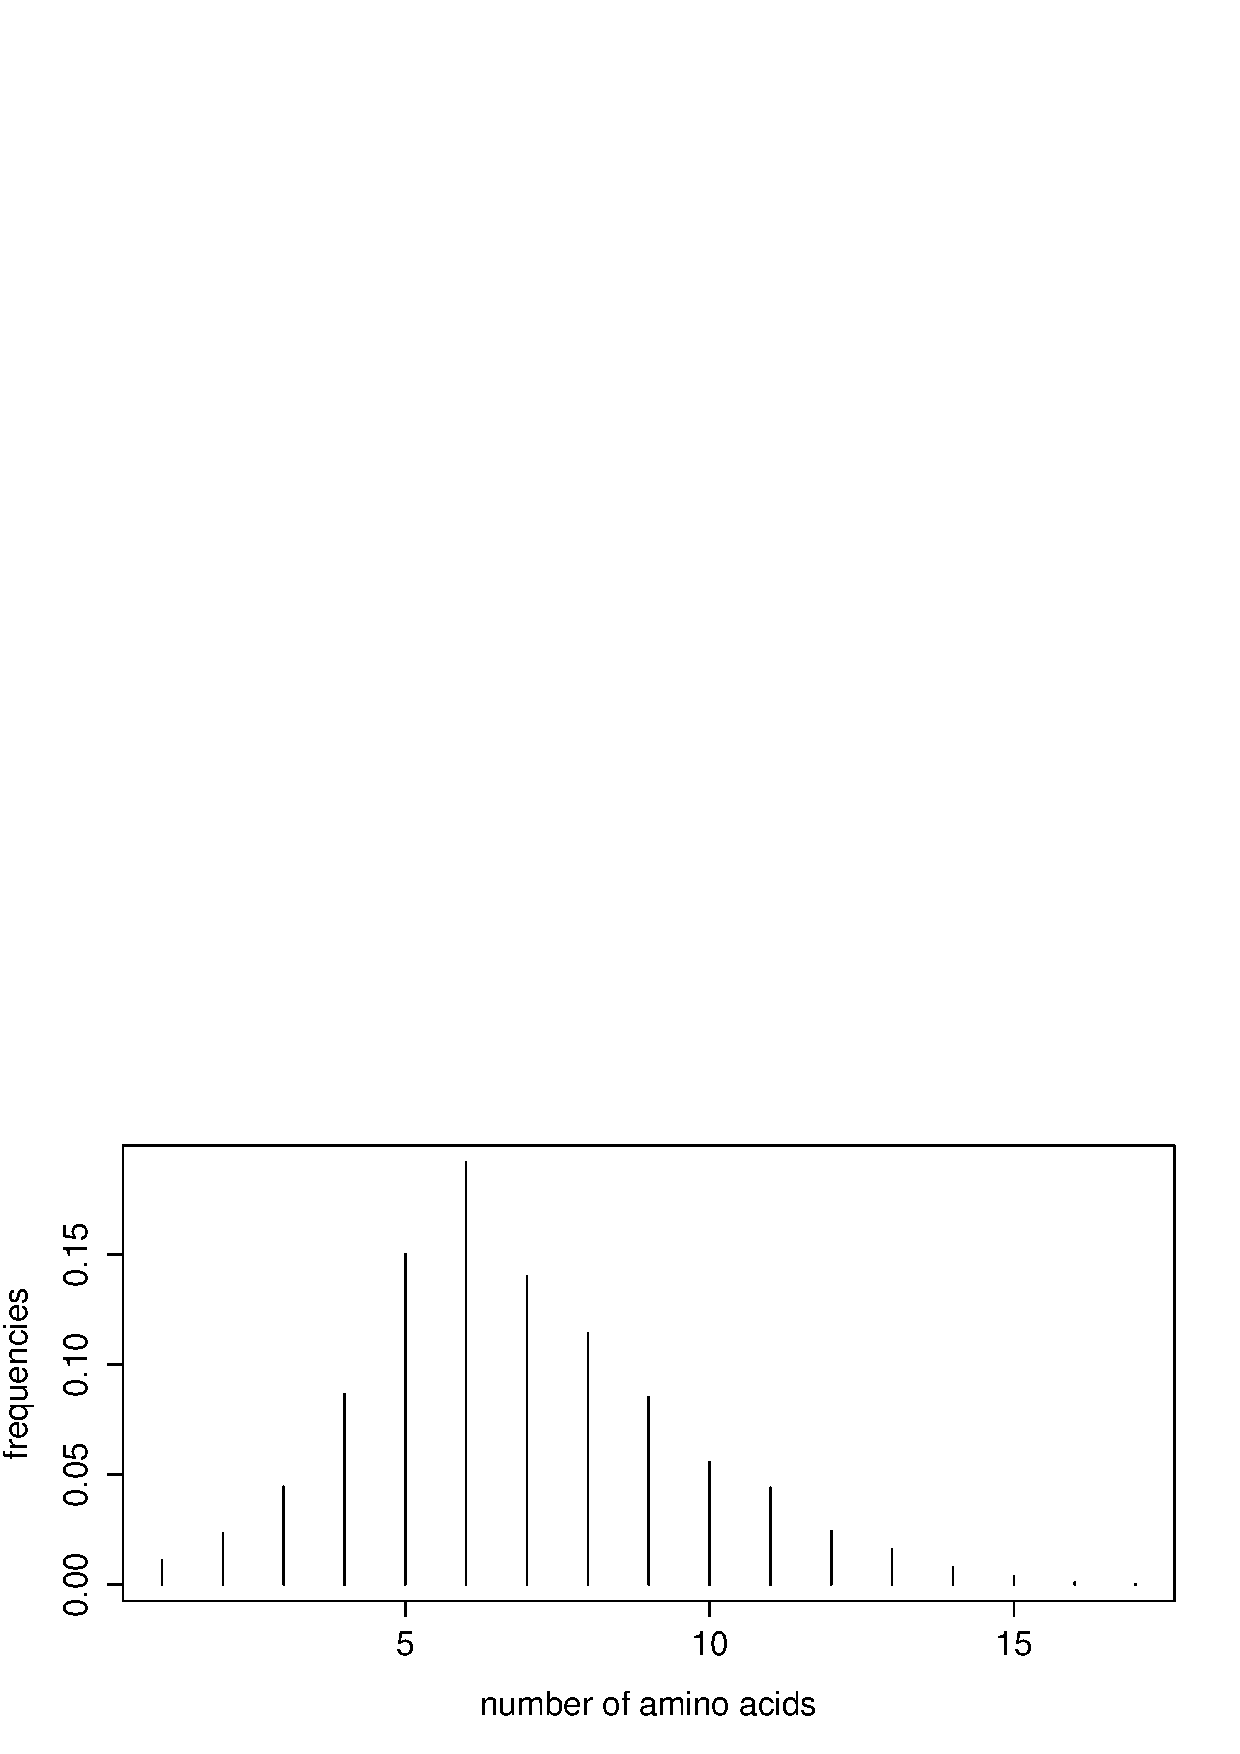
\includegraphics[width=\textwidth]{AAnum.pdf}
\label{fig:AAnum}
\end{figure}


\begin{figure}[h]
\caption{Density plot of percentages of the likelihood achieved by the optimal amino acid found by max rule.}
\centering
\includegraphics[width=\textwidth]{percentile.pdf}
\label{fig:percentile}
\end{figure}


%\subsubsection{Model accuracy}
%To assess model accuracy, we did simulations using the maximum likelihood estimates from Rokas et. al. 's data. (waiting on results)

\subsection{Simulated data vs. observed data}
We also evaluate the models by simulating data under models and comparing them with the observed data. 
First, a single taxon (Scas) is deleted from the Rokas's yeast gene tree, model parameters are estimated from the data on the remaining taxa. 
Then the ancestral sequence where the missing taxon is attached is estimated, where the probabilities of observing all 20 amino acids at each site are calculated. 
Then the deleted data is put back and the length of the truncated branch earlier is estimated using the parameters on the pruned tree. 
With the parameter values, the length of the missing branch, and the sequence at the start of the branch, we simulate the evolution of a gene's coding sequence from the reconstructed taxon to the deleted taxon from our analysis.
We then compare the simulated sequence at the deleted taxon with the real data. 
\begin{figure}[h]
\centering
\includegraphics[width=\textwidth]{simulation.png}
\label{fig:simulation}
\end{figure}
The results are shown in Figure \ref{fig:simulation}. 
On the left, each dot represents the proportion of amino acids that differ between the simulated and the observed sequence for a given gene. 
Our new model performed much better than the standard WAG model in matching sequences, especially for genes under high selection that are shown in brighter dots. 
On the right repeated simulations are plotted under our new model (red) and WAG model (blue) starting from the ancestral sequence estimated under the estimated sequences under the new model (upper lines) and WAG model (lower lines) for a single gene. 
The dotted line represents the functionality for the observed sequence.
When the ancestral sequences are estimated from WAG model, they have much lower fitnesses. 
If evolved under WAG model, the fitness does not improve much at the end of the branch.
On the other hand there is directional selection leading to an increase in fitness if the sequences evolve under the new model. 
When the ancestral sequences are estimated from the new model the fitness is significantly higher. 
And WAG simulation leads to a decrease in fitness while the fitness is maintained under simulation with the new model.
No matter how the ancestral sequences are obtained, the new model presents a better match to the observed data.
This realistic behavior shows that the new model is more adequate than the WAG model for Rokas's data. [I THINK WE SHOULD USE THE ACTUAL BEST MODEL UNDER PROTTEST, PLUS  AA BASED ON GY94 AND GTR CODON/NUCLEOTIDE MODELS]


%%%%%%%%%%%%%%%%%%%%%%%%%%%%%%%%%%%%%%%%%%%%%%%%%%%%%%%%
\newpage
\bibliographystyle{plainnat}
\bibliography{ProEvo}
\end{document}